\documentclass[12pt]{article}\usepackage[]{graphicx}\usepackage[]{color}
%% maxwidth is the original width if it is less than linewidth
%% otherwise use linewidth (to make sure the graphics do not exceed the margin)
\makeatletter
\def\maxwidth{ %
  \ifdim\Gin@nat@width>\linewidth
    \linewidth
  \else
    \Gin@nat@width
  \fi
}
\makeatother

\definecolor{fgcolor}{rgb}{0.345, 0.345, 0.345}
\newcommand{\hlnum}[1]{\textcolor[rgb]{0.686,0.059,0.569}{#1}}%
\newcommand{\hlstr}[1]{\textcolor[rgb]{0.192,0.494,0.8}{#1}}%
\newcommand{\hlcom}[1]{\textcolor[rgb]{0.678,0.584,0.686}{\textit{#1}}}%
\newcommand{\hlopt}[1]{\textcolor[rgb]{0,0,0}{#1}}%
\newcommand{\hlstd}[1]{\textcolor[rgb]{0.345,0.345,0.345}{#1}}%
\newcommand{\hlkwa}[1]{\textcolor[rgb]{0.161,0.373,0.58}{\textbf{#1}}}%
\newcommand{\hlkwb}[1]{\textcolor[rgb]{0.69,0.353,0.396}{#1}}%
\newcommand{\hlkwc}[1]{\textcolor[rgb]{0.333,0.667,0.333}{#1}}%
\newcommand{\hlkwd}[1]{\textcolor[rgb]{0.737,0.353,0.396}{\textbf{#1}}}%
\let\hlipl\hlkwb

\usepackage{framed}
\makeatletter
\newenvironment{kframe}{%
 \def\at@end@of@kframe{}%
 \ifinner\ifhmode%
  \def\at@end@of@kframe{\end{minipage}}%
  \begin{minipage}{\columnwidth}%
 \fi\fi%
 \def\FrameCommand##1{\hskip\@totalleftmargin \hskip-\fboxsep
 \colorbox{shadecolor}{##1}\hskip-\fboxsep
     % There is no \\@totalrightmargin, so:
     \hskip-\linewidth \hskip-\@totalleftmargin \hskip\columnwidth}%
 \MakeFramed {\advance\hsize-\width
   \@totalleftmargin\z@ \linewidth\hsize
   \@setminipage}}%
 {\par\unskip\endMakeFramed%
 \at@end@of@kframe}
\makeatother

\definecolor{shadecolor}{rgb}{.97, .97, .97}
\definecolor{messagecolor}{rgb}{0, 0, 0}
\definecolor{warningcolor}{rgb}{1, 0, 1}
\definecolor{errorcolor}{rgb}{1, 0, 0}
\newenvironment{knitrout}{}{} % an empty environment to be redefined in TeX

\usepackage{alltt}
\usepackage[utf8]{inputenc}
\usepackage{amsmath}
\usepackage{fullpage}
\usepackage{enumitem}
\usepackage{graphicx}
\usepackage{fancyhdr}
\usepackage{setspace}
\usepackage{titlesec}
\usepackage{caption}
\pagestyle{fancy}
\lhead{Justin Gomez, Paul Harmon}
\chead{Data Analysis Proposal}
\rhead{March 30, 2017}
\setlength{\headheight}{20pt}
\renewcommand{\headrulewidth}{0.2pt}
\renewcommand{\footrulewidth}{0.2pt}
\setlength{\parindent}{0pt}
\IfFileExists{upquote.sty}{\usepackage{upquote}}{}
\begin{document}



\doublespacing

\section{Background}
NCAA College Basketball, including the regular season and the NCAA tournament, is a major cornerstone of college sports. Each year, from mid-November to mid-March, the best Men’s and Women’s college basketball teams face off against each other. Each teams’ season culminates in a bid to enter the either the NCAA tournament or its subsidiary, the NIT. While the games themselves have tremendous economic impact, college basketball's effects reach beyond the court. Broadcasting the tournament cost CBS nearly 10 billion dollars in 2016 (Forbes). The effect on the schools’ academics is palpable, too; Smith (2008) notes that “a college’s profile will increase with big-time athletics, as will the perception of the school itself”. Indeed, some have even contended the increased visibility has impacts on academic metrics at those schools including increased student quality and retention.\\

Naturally, methods for accurately picking winners and losers of college basketball games are of interest for several reasons. For fans, predictive models can aid in filling out brackets in early March. For coaches, better understanding which factors influence the outcome of a game can help them understand how better to develop game plans and coach student athletes to victory. While much work has been done in the field of predictive analytics related to the NCAA tournament, much focus is placed on "black box" predictive algorithms or complex regression schemes. This analysis instead focuses mainly on the development of a binary regression model in order determine which factors may influence the probability of a home team winning a given basketball game.\\


\section{Data Set Description}
The data were obtained from a repository on Kaggle.com related to the March Machine Learning Mania competition in 2016. A great deal of information was originally pulled down, much more than we could ever use in any meaningful way. In the end, we have settled on fourteen predictor variables to include in our study of our single response: whether the home team won or not. Our data set contains more than sixty-four thousand games spanning fourteen seasons of basketball. Team rosters are continuously changing as students enter and leave programs for a myriad of reasons. This leads to teams being relatively unchanged within a single year, but year to year we could see very different teams, so it seems to make sense to account for this behind the scenes shift by adding a season variable to our model. Whether or not a game goes into overtime is also a variable of interest as it may provide some insight into the level of competition between the teams; games that go into overtime likely involve more evenly matched teams than those that do not, and thus the probability of the home team winning may be close to 50\%. To get an idea for how many points winning teams might need to put up in a typical game, we will also include the winning team's score.From there, our data consists of performance statistics for both teams summarized as either percentages or differentials. For percentage predictors, we have field goal, three-point, and free-throw percentages for both the winning and the losing teams. All percentages were calculated as the number of made shots divided by the number of atempted shots. Next, are our differentials. We will be considering total rebounds (offensive rebounds plus defenseive rebounds), assists, turnovers, steals, blocks, and personal fouls when calculating these differentials, and we will always subtract the losing team's game statistics from the winning team's (winner-loser).

\section{Goals and Questions of Interest}
We are interested in determining the factors that influence the outcomes of college basketball games in order to predict which teams are more likely to win a matchup. The key questions of interest are as follows.

\begin{enumerate}
\item %1
Does home court advantage influence the outcome of a game, after controlling for on-court performance factors?

\item %2
Do winning teams turn the ball over less than losing teams?

\item %3
Do any of the variables measured modify the effect of other covariates of interest?

\end{enumerate}

The key goal of the analysis is to create a good predictive model that can, generate predictions as to whether a team will win or lose a game.  We plan to break the dataset into training and testing sets in order to assess the quality of predictions.  Since the data pertain to multiple seasons, the training and testing sets are going to be chosen using a stratified random sampling method that evenly samples games form each season. 

\section{Preliminary Data Exploartion}
Before building any models or jumping into the heavy analysis, we can create several plots that give us some insight into the data. Understanding the existing structure (or lack of) within our predictors may help us decide how to incorporate variables in our model, if at all. To get at these relationships, a simple correlation matrix has been calculated and summarized in Figure~\ref{fig:corr}.

\begin{figure}[h]
\centering
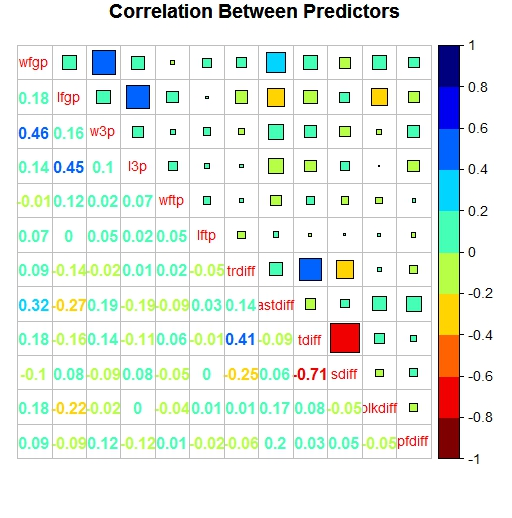
\includegraphics[width=.7\textwidth]{correlations.jpeg}
\captionsetup{font=footnotesize,labelfont=footnotesize}
\caption{\label{fig:corr} \textbf{Correlation plot for the set of predictors. Size and color of the square gives a general idea of the size and direction of the relationship while the lower triangle gives actual values.}}
\end{figure}

While many relationships are not as strong as we initially expected, there are not many surprises in this plot. Field goal percentage and three-point percentage are fairly strongly correlated for winning and losing teams, which makes sense as three-pointers are a subset of overall field goals. We also see a large negative correlation between turnover differential and steal differential, which is expected as the winning team should turn the ball over less, but steal the ball more. With this information, we might be able to justify leaving out a variable or two, but for the most part, the low correlations present between this set of variables indicate that including all variables in a model initially isn't a bad idea.\\

We can also examine a series of plots that examine the differentials specifically and how they relate to whether the home team won or not in Figure~\ref{fig:diff}. These plots show the proportion of games won for teams that had a negative differential vs. a positive differential. For offensive statistics, such as assists, steals, and blocks, teams that had a positive differential were more likely to win. This makes sense; a team with a positive assist differential had more assists than the other team, so it is likely that they ought to have scored more points than the other team as well. Not surprisingly, teams with negative turnover differentials were actually more likely to win than teams with positive turnover differentials (because they turned the ball over fewer times than their opponent) and teams that fouled less were more likely to win. These plots ought to inform some intuition about the direction of the coefficients estimated in the binary regression. \\

\begin{figure}[h]
\centering
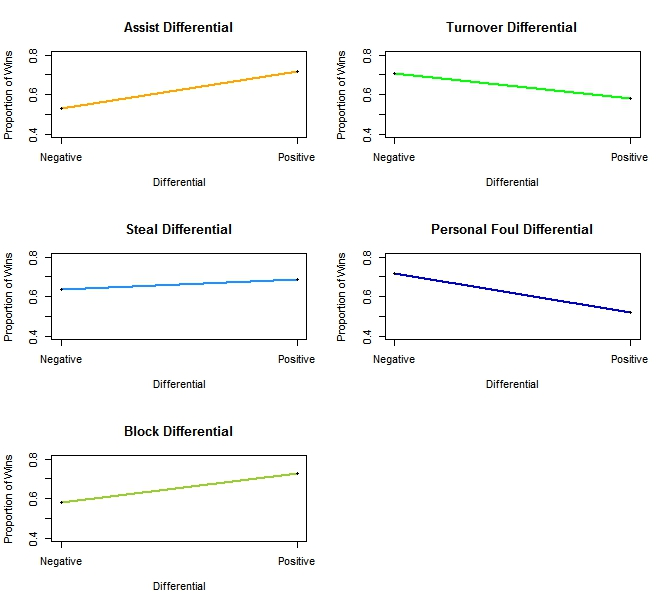
\includegraphics[width=.7\textwidth]{differentials.jpeg}
\captionsetup{font=footnotesize,labelfont=footnotesize}
\caption{\label{fig:diff} \textbf{Plots of the five differential variables being considered as predictors. Proportions of wins are evaluated for winning teams with positive and negative differentials on each variable. Differentials found as winning minus losing.}}
\end{figure}


\section{Analysis Plan and Modeling}

We will focus on methods designed for binary regression models. We plan on using logistic regression to analyze the data. The choice of link function is not one that we have decided on yet; choosing between a logit link or a probit link may be one of the key questions we answer. The logit makes sense because we could interpret the direct change in the odds of winning given a change in one of the covariates. However, the probit might be worth looking into as well. We could think of the outcome of a basketball game as being the result of some underlying latent index of player performance. 

In any case, the plan for modeling this be as follows. We will fit models with the response, whether or not the home team won, and determine which combinations of covariates form the most parsimonious model. We can then start to use that model to assess the research questions we came up with:

\begin{enumerate}
\item %1
Based on the structure of the response (home games won), probably the best way to assess this question would be to fit models and make predictions. We plan to fit models on a training set and test on validation set. 

\item %2
The turnover differential term will be retained in the model, since it is a specific question we want to answer. We will perform hypothesis tests and confidence intervals for the effect of turnover differential on win probability.
\item %3
Testing for effect modifiers would be done by including interaction terms in the model. It might be interesting to see if the effects of covariates on the probability of winning are the same in games that go to overtime vs. those that do not.  

\end{enumerate}

The model fitting should not be overly complicated in this analysis. The final step will include using the testing set to determine whether the predictive logisitic model we created is effective for predicting the outcome of a college basketball game. 

\section{Sources}
Smith, D. Randall. (2008) Big Time College Basketball and the Advertising Effect: Does Success Really Matter? Journal of Sports Economics Volume 9 No. 4 pp 387-406.

Ogus, Simon. (2016) The Economic Impact of March Madness From First Four to Final Four. Forbes. 

\end{document}
